\newpage
    \subsection{Task 1.3}
    \subsubsection{Draw a use-case diagram for the whole system}
    \begin{center}
    \begin{figure}[htp]
    \begin{center}
     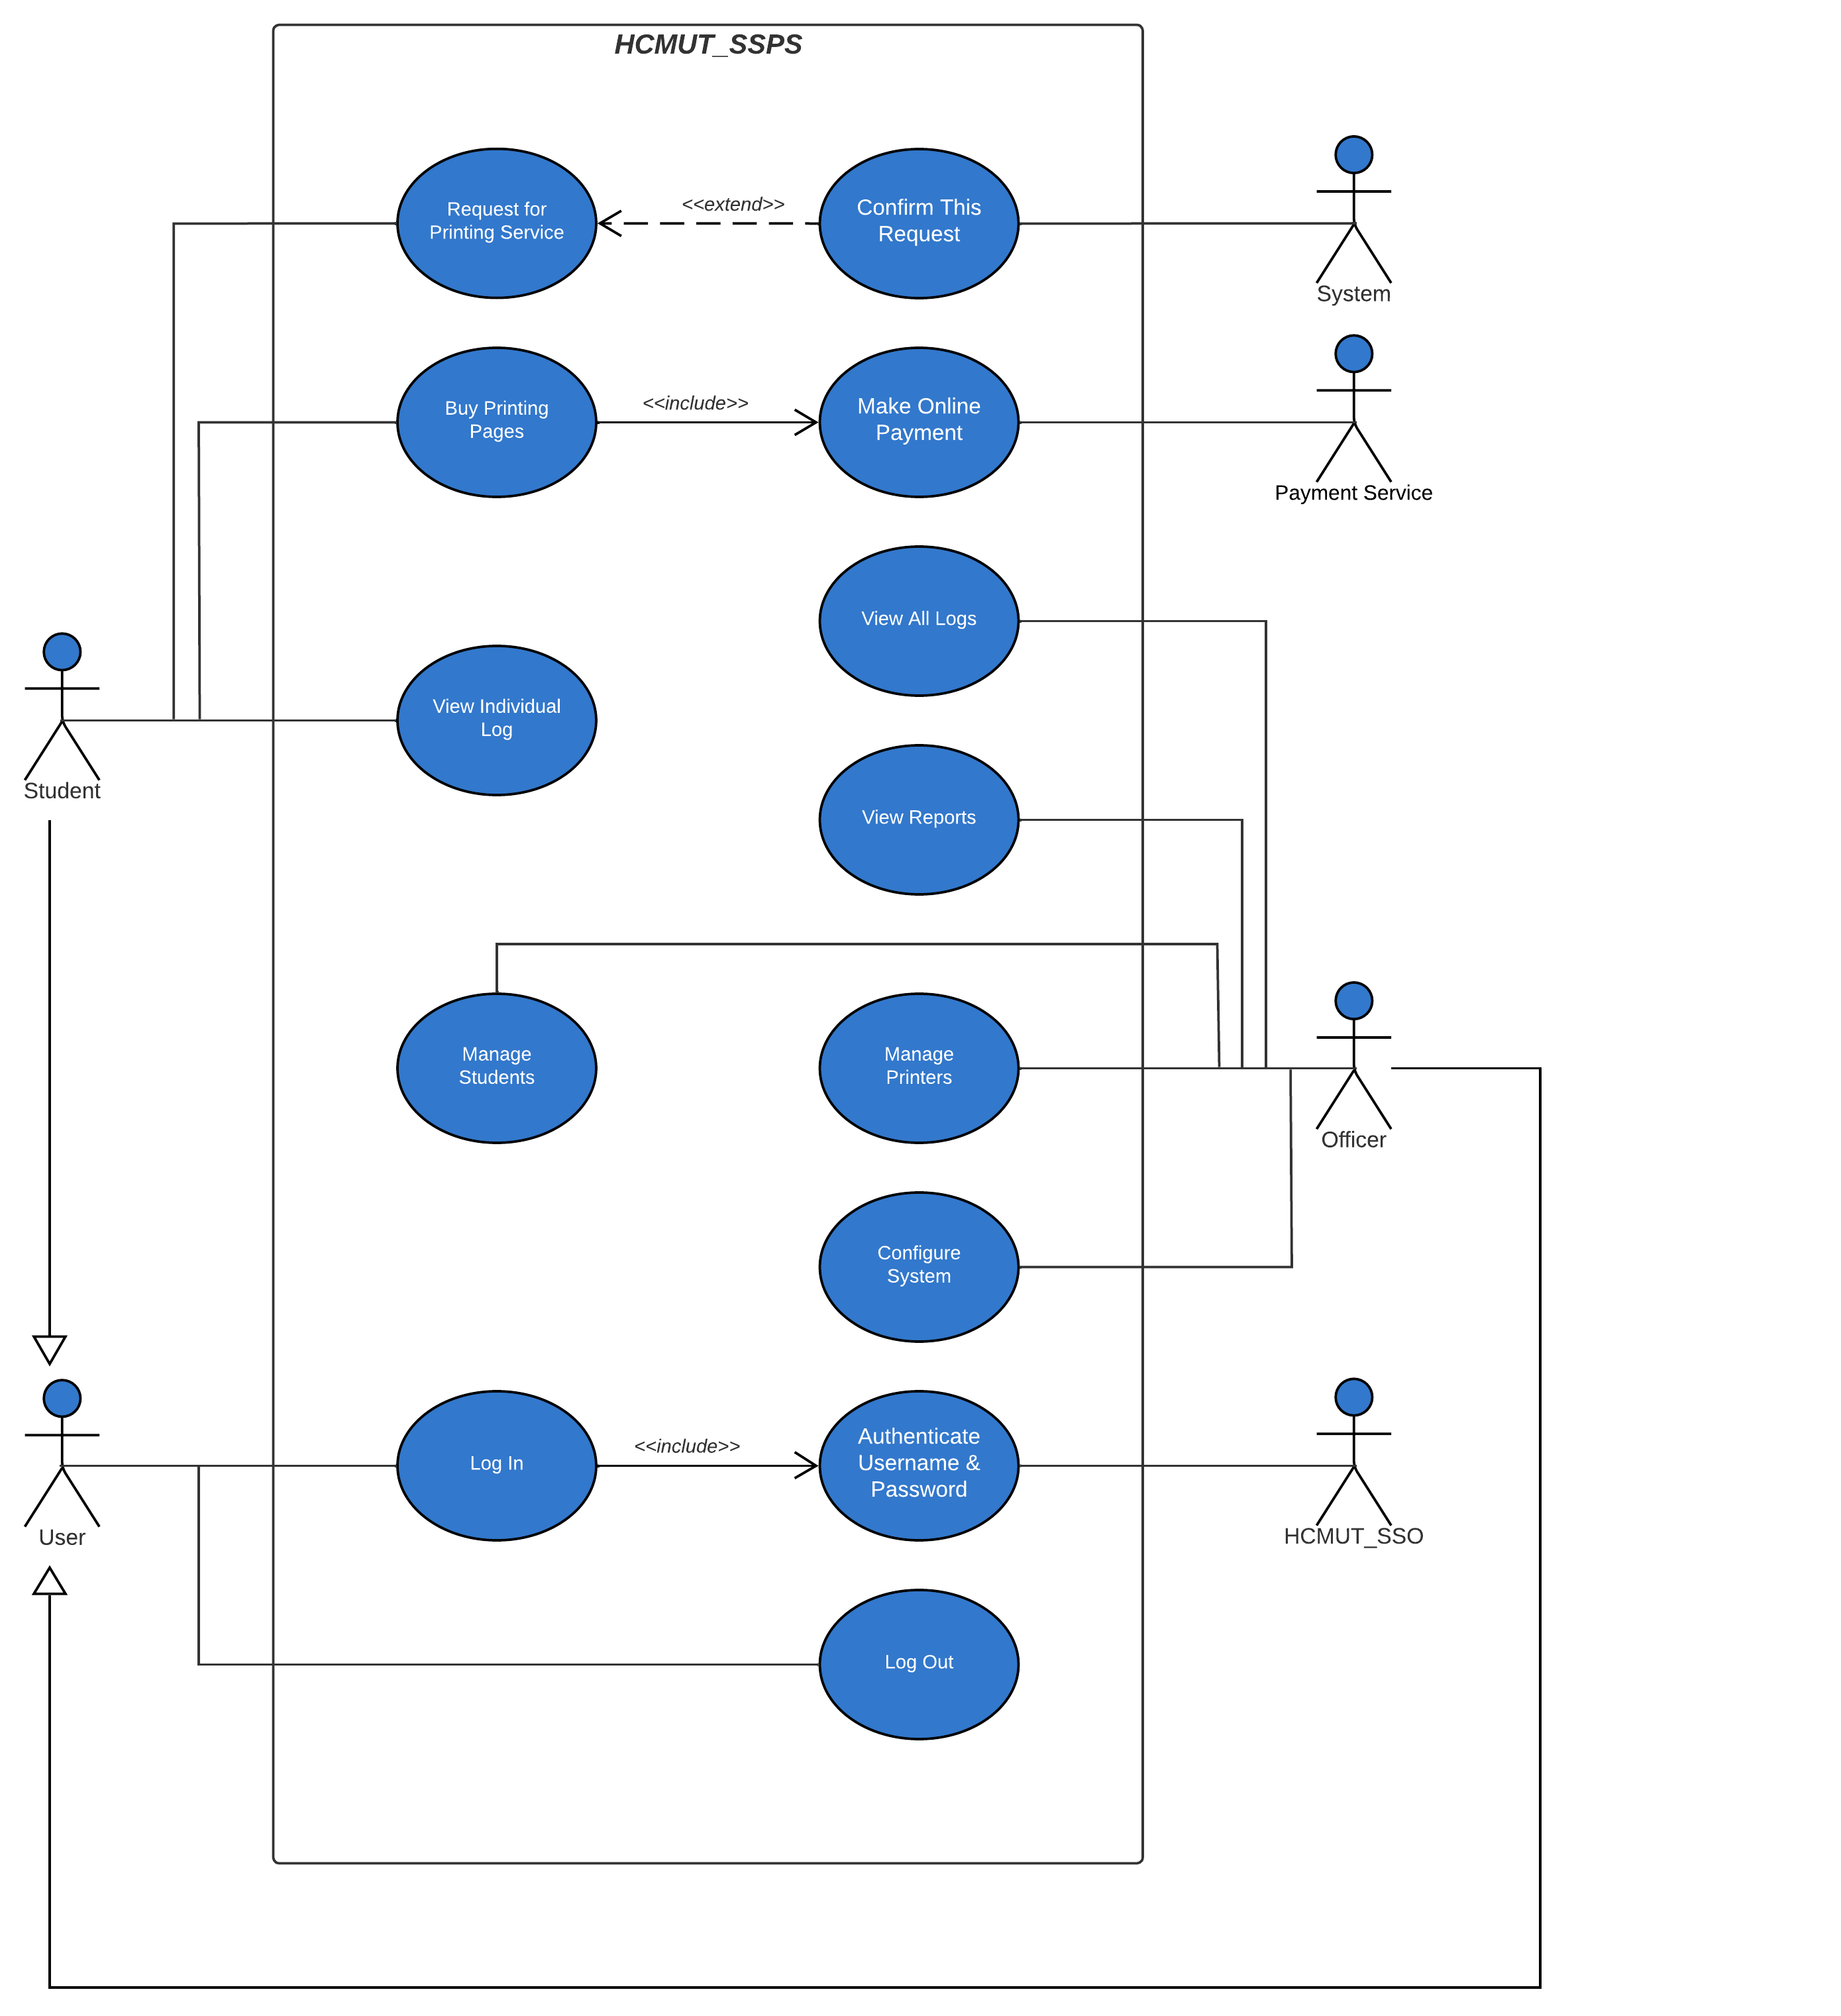
\includegraphics[scale=.62]{images/Task1/wholeSystem.png}
    \end{center}
    \label{refhinh1}
    \end{figure}
    \end{center}

    \newpage
    \subsubsection{Choose an important module and draw its use-case diagram, as well as describe the use-case using a table format}

    \begin{enumerate}[a)]
    \item {\textbf{Request for Printing Service}}
    \begin{center}
    \begin{figure}[htp]
    \begin{center}
     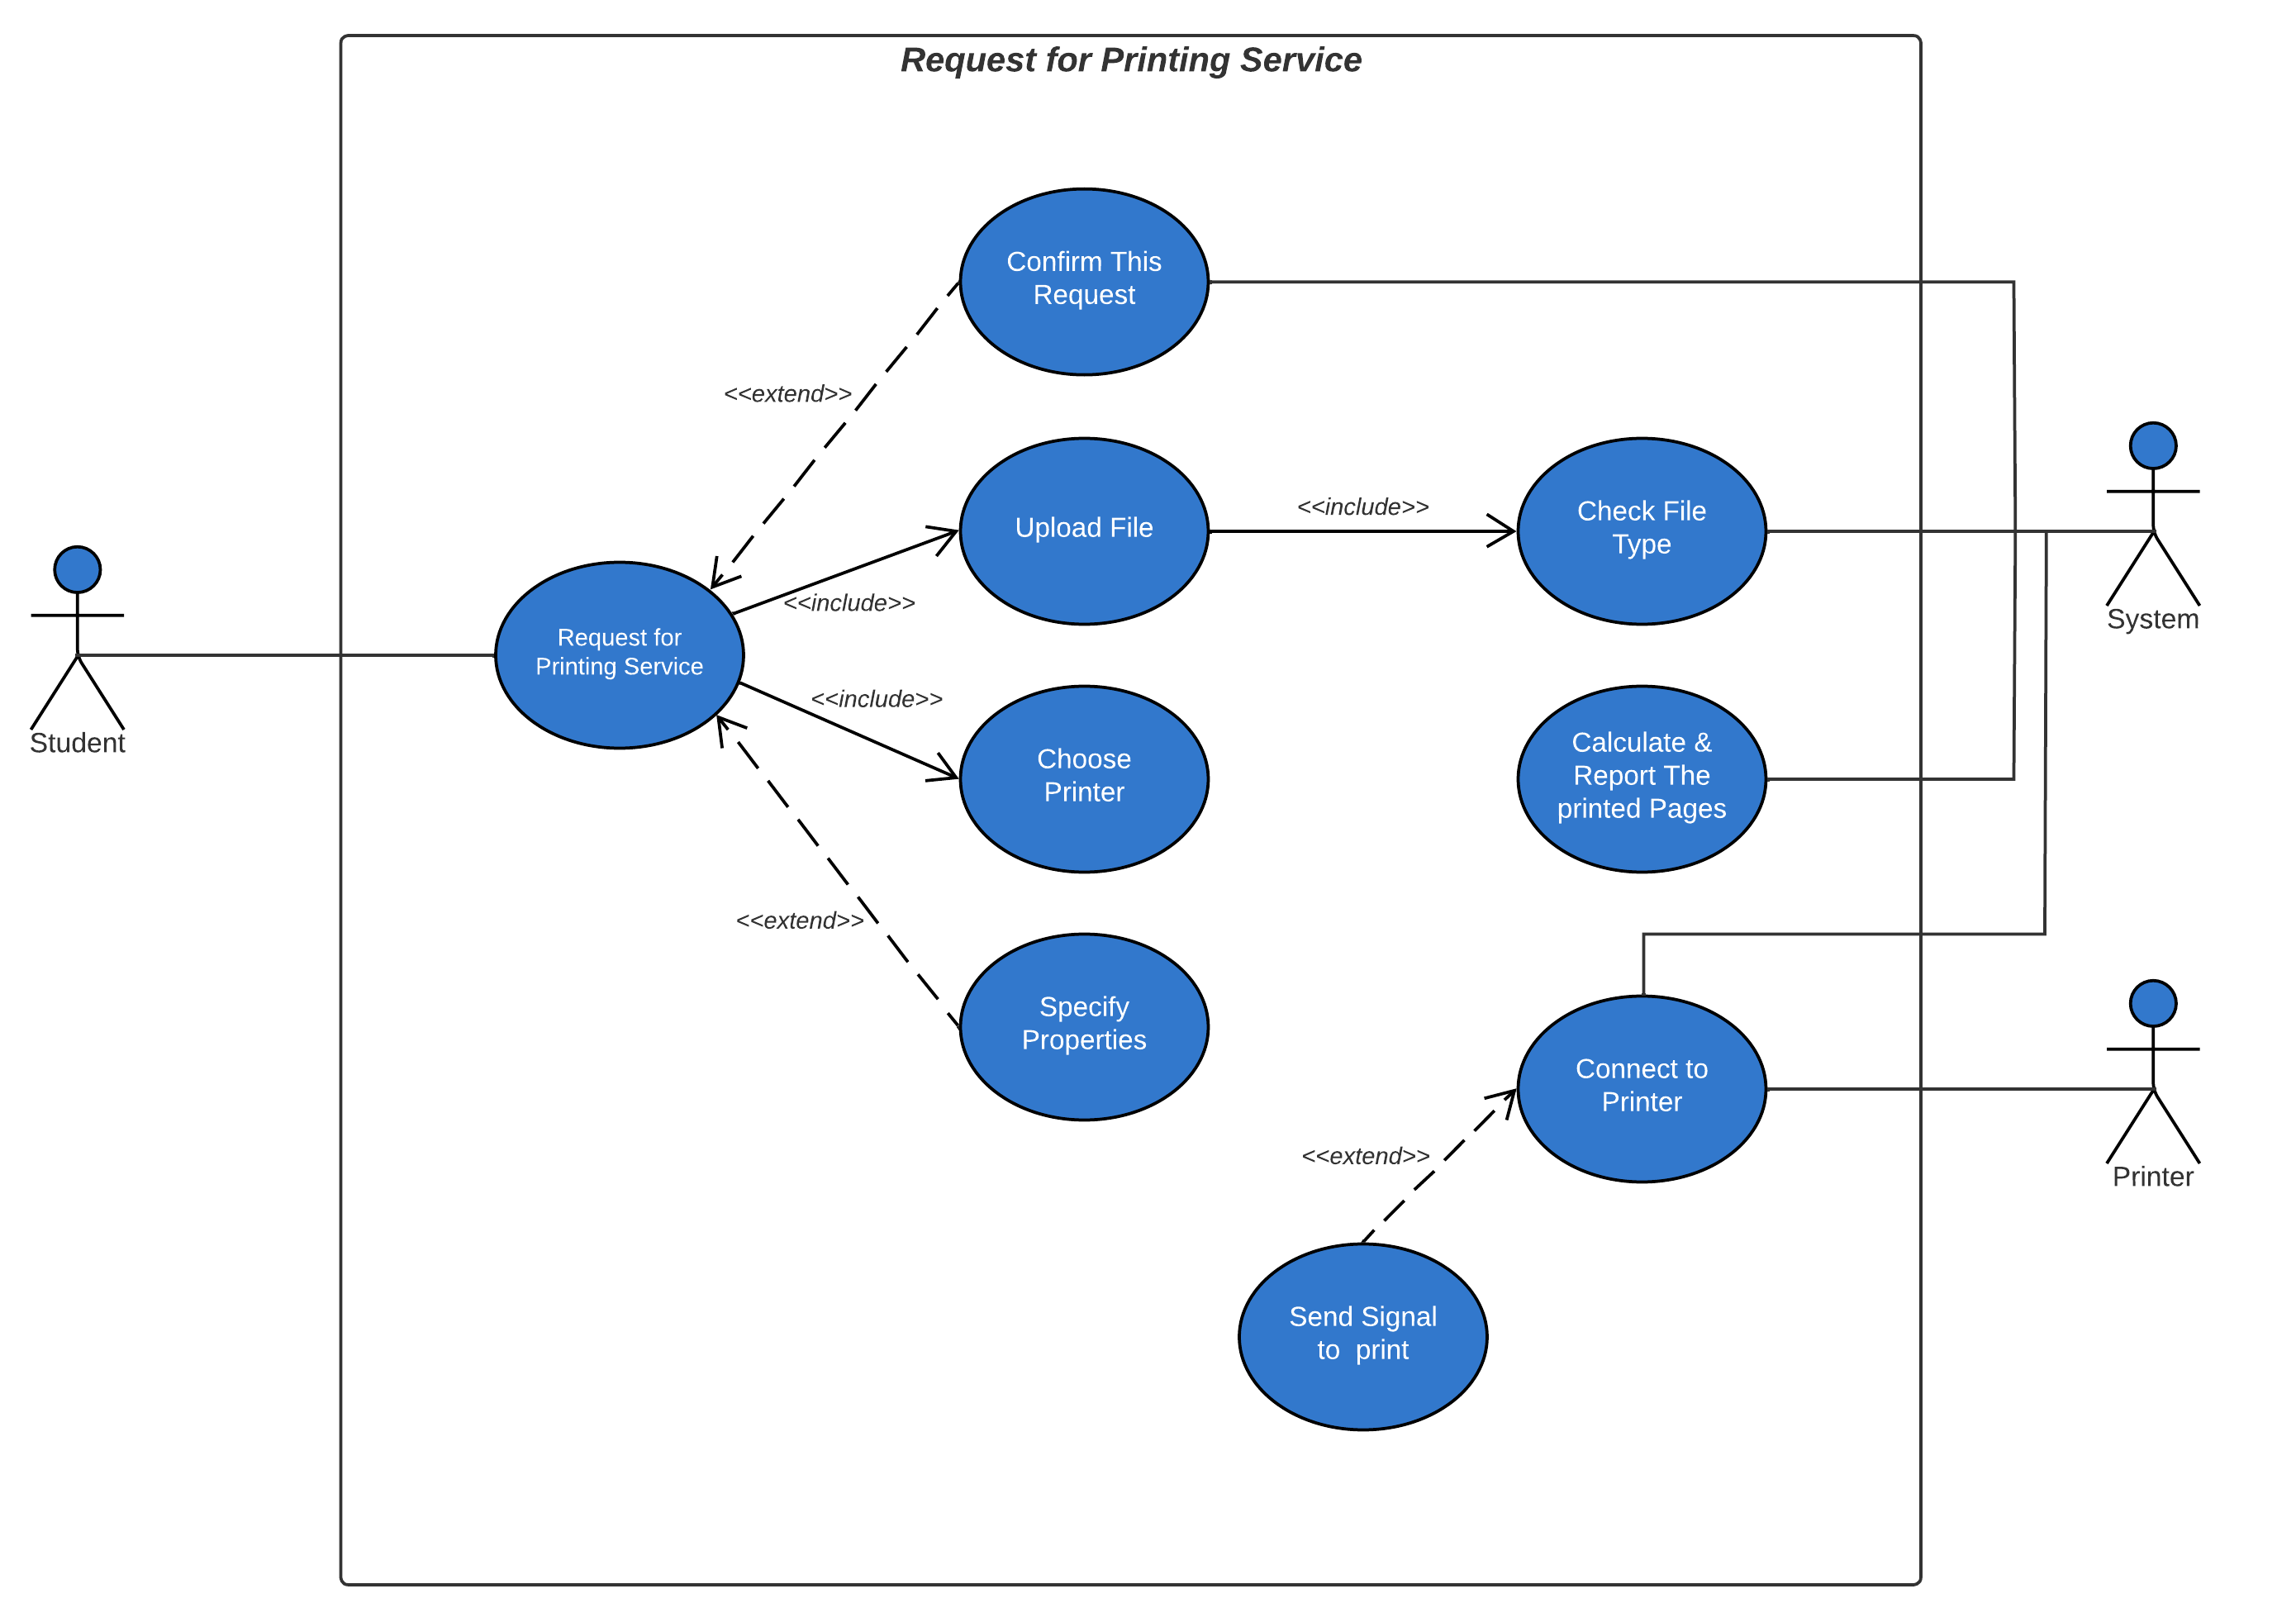
\includegraphics[scale=.62]{images/Task1/requestForPrintingService.png}
    \end{center}
    \label{refhinh1}
    \end{figure}
    \end{center}

    \begin{longtable}{|l|p{10cm}|}
        \hline
        \endhead
        \hline
        \endfoot
        Use-case Name & \textbf{Request for Printing Service}\\
        \hline
        Actors & Sinh viên.\\
        \hline
        Description & Sinh viên sử dụng chức năng này để tiến hành thực hiện in tài liệu thông qua hệ thống máy in của nhà trường.\\
        \hline
        Trigger & Sinh viên nhấn vào nút "In tài liệu".\\
        \hline
        Pre-conditions & Sinh viên đăng nhập vào hệ thống thành công.\\
        \hline
        Post-conditions & None.\\
        \hline
        Basic Flow & 1. Sinh viên chọn mục "Dịch vụ".\\
        & 2. Sinh viên chọn "In tài liệu".\\
        & 3. Hệ thống hiển thị các trường thông tin mà sinh viên cần phải cung cấp.\\
        & 4. Sinh viên tải tài liệu cần in lên hệ thống.\\
        & 5. Hệ thống kiểm tra loại tài liệu sinh viên cung cấp có thuộc một trong các loại được hệ thống cho phép hay không.\\
        & 6. Sinh viên chọn máy in mà mình muốn kết nối để sử dụng.\\
        & 7. Các thuộc tính in sẽ có giá trị mặc định. Tuy nhiên, sinh viên có thể điều chỉnh lại các thuộc tính in này cho phù hợp với nhu cầu.\\
        & 8. Sinh viên nhấn vào nút "Hoàn tất" để hoàn thành các tuỳ chọn.\\
        & 9. Hệ thống hiển thị tổng quát các thông tin mà sinh viên đã cung cấp.\\
        & 10. Sinh viên nhấn vào nút "Tiến hành in" để xác nhận gửi yêu cầu in tài liệu đến hệ thống.\\
        & 11. Hệ thống tiếp nhận và xử lý yêu cầu. Hệ thống sẽ tính toán số lượng trang in miễn phí còn lại của mỗi sinh viên và thông báo số lượng trang in mà sinh viên cần mua thêm.\\ 
        & 12. Hệ thống thông báo dịch vụ in được xác nhận thành công và tiến hành in tài liệu cho sinh viên.\\

        \hline
        Alternative Flow & Alternative 1: Sau bước 4,  nếu tài liệu được tải lên không hợp lệ:\\
        & \hspace{1em} 4.1. Hệ thống hiện thông báo "Tài liệu này có định dạng không hợp lệ. Vui lòng chọn một tài liệu khác!".\\
        & \hspace{1em} 4.2. Sinh viên chọn "Đồng ý" để quay lại bước 4 trong \textit{Basic Flow} và tải lên lại một tài liệu khác.\\
        &\\
        & Alternative 2: Sau bước 8, nếu có ít nhất một trong các trường thông tin bị để trống:\\
        & \hspace{1em} 8.1. Hệ thống thông báo việc gửi yêu cầu in của sinh viên thất bại và chỉ ra những trường thông tin còn trống đó.\\
        & \hspace{1em} 8.2. Sinh viên cung cấp đầy đủ các thông tin mà hệ thống yêu cầu và quay lại bước 7 trong \textit{Basic Flow}.\\
         &\\
        & Alternative 3: Sau bước 9, nếu một số thông tin về dịch vụ cần được thay đổi:\\
        & \hspace{1em} 9.1. Sinh viên chọn "Quay lại" để quay về bước 4 trong \textit{Basic Flow} để điều chỉnh lại các thông tin cho phù hợp.\\
        &\\
        & Alternative 4: Sau bước 11, nếu số lượng trang in cần cho yêu cầu in hiện tại vượt quá số lượng trang in miễn phí còn lại của sinh viên:\\
        & \hspace{1em} 11.1. Sinh viên chọn "Mua thêm" để sử dụng tính năng mua thêm trang in (Buy Printing Pages) và tiếp tục bước 12 trong \textit{Basic Flow}.\\
        \hline
        Exception Flow & Exception 1: Sau bước 4.1, sinh viên có thể chọn "Thoát" để huỷ dịch vụ in và trở về trang chủ.\\
        &\\
        & Exception 2: Sau bước 8.1, sinh viên có thể chọn "Thoát" để huỷ dịch vụ in và trở về trang chủ.\\
        &\\
        & Exception 3: Sau bước 11.1, sinh viên có thể chọn "Thoát" để huỷ dịch vụ in và trở về trang chủ.\\
    \end{longtable}

    \newpage
    \item{\textbf{Make Online Payment}}
    \begin{center}
    \begin{figure}[htp]
    \begin{center}
     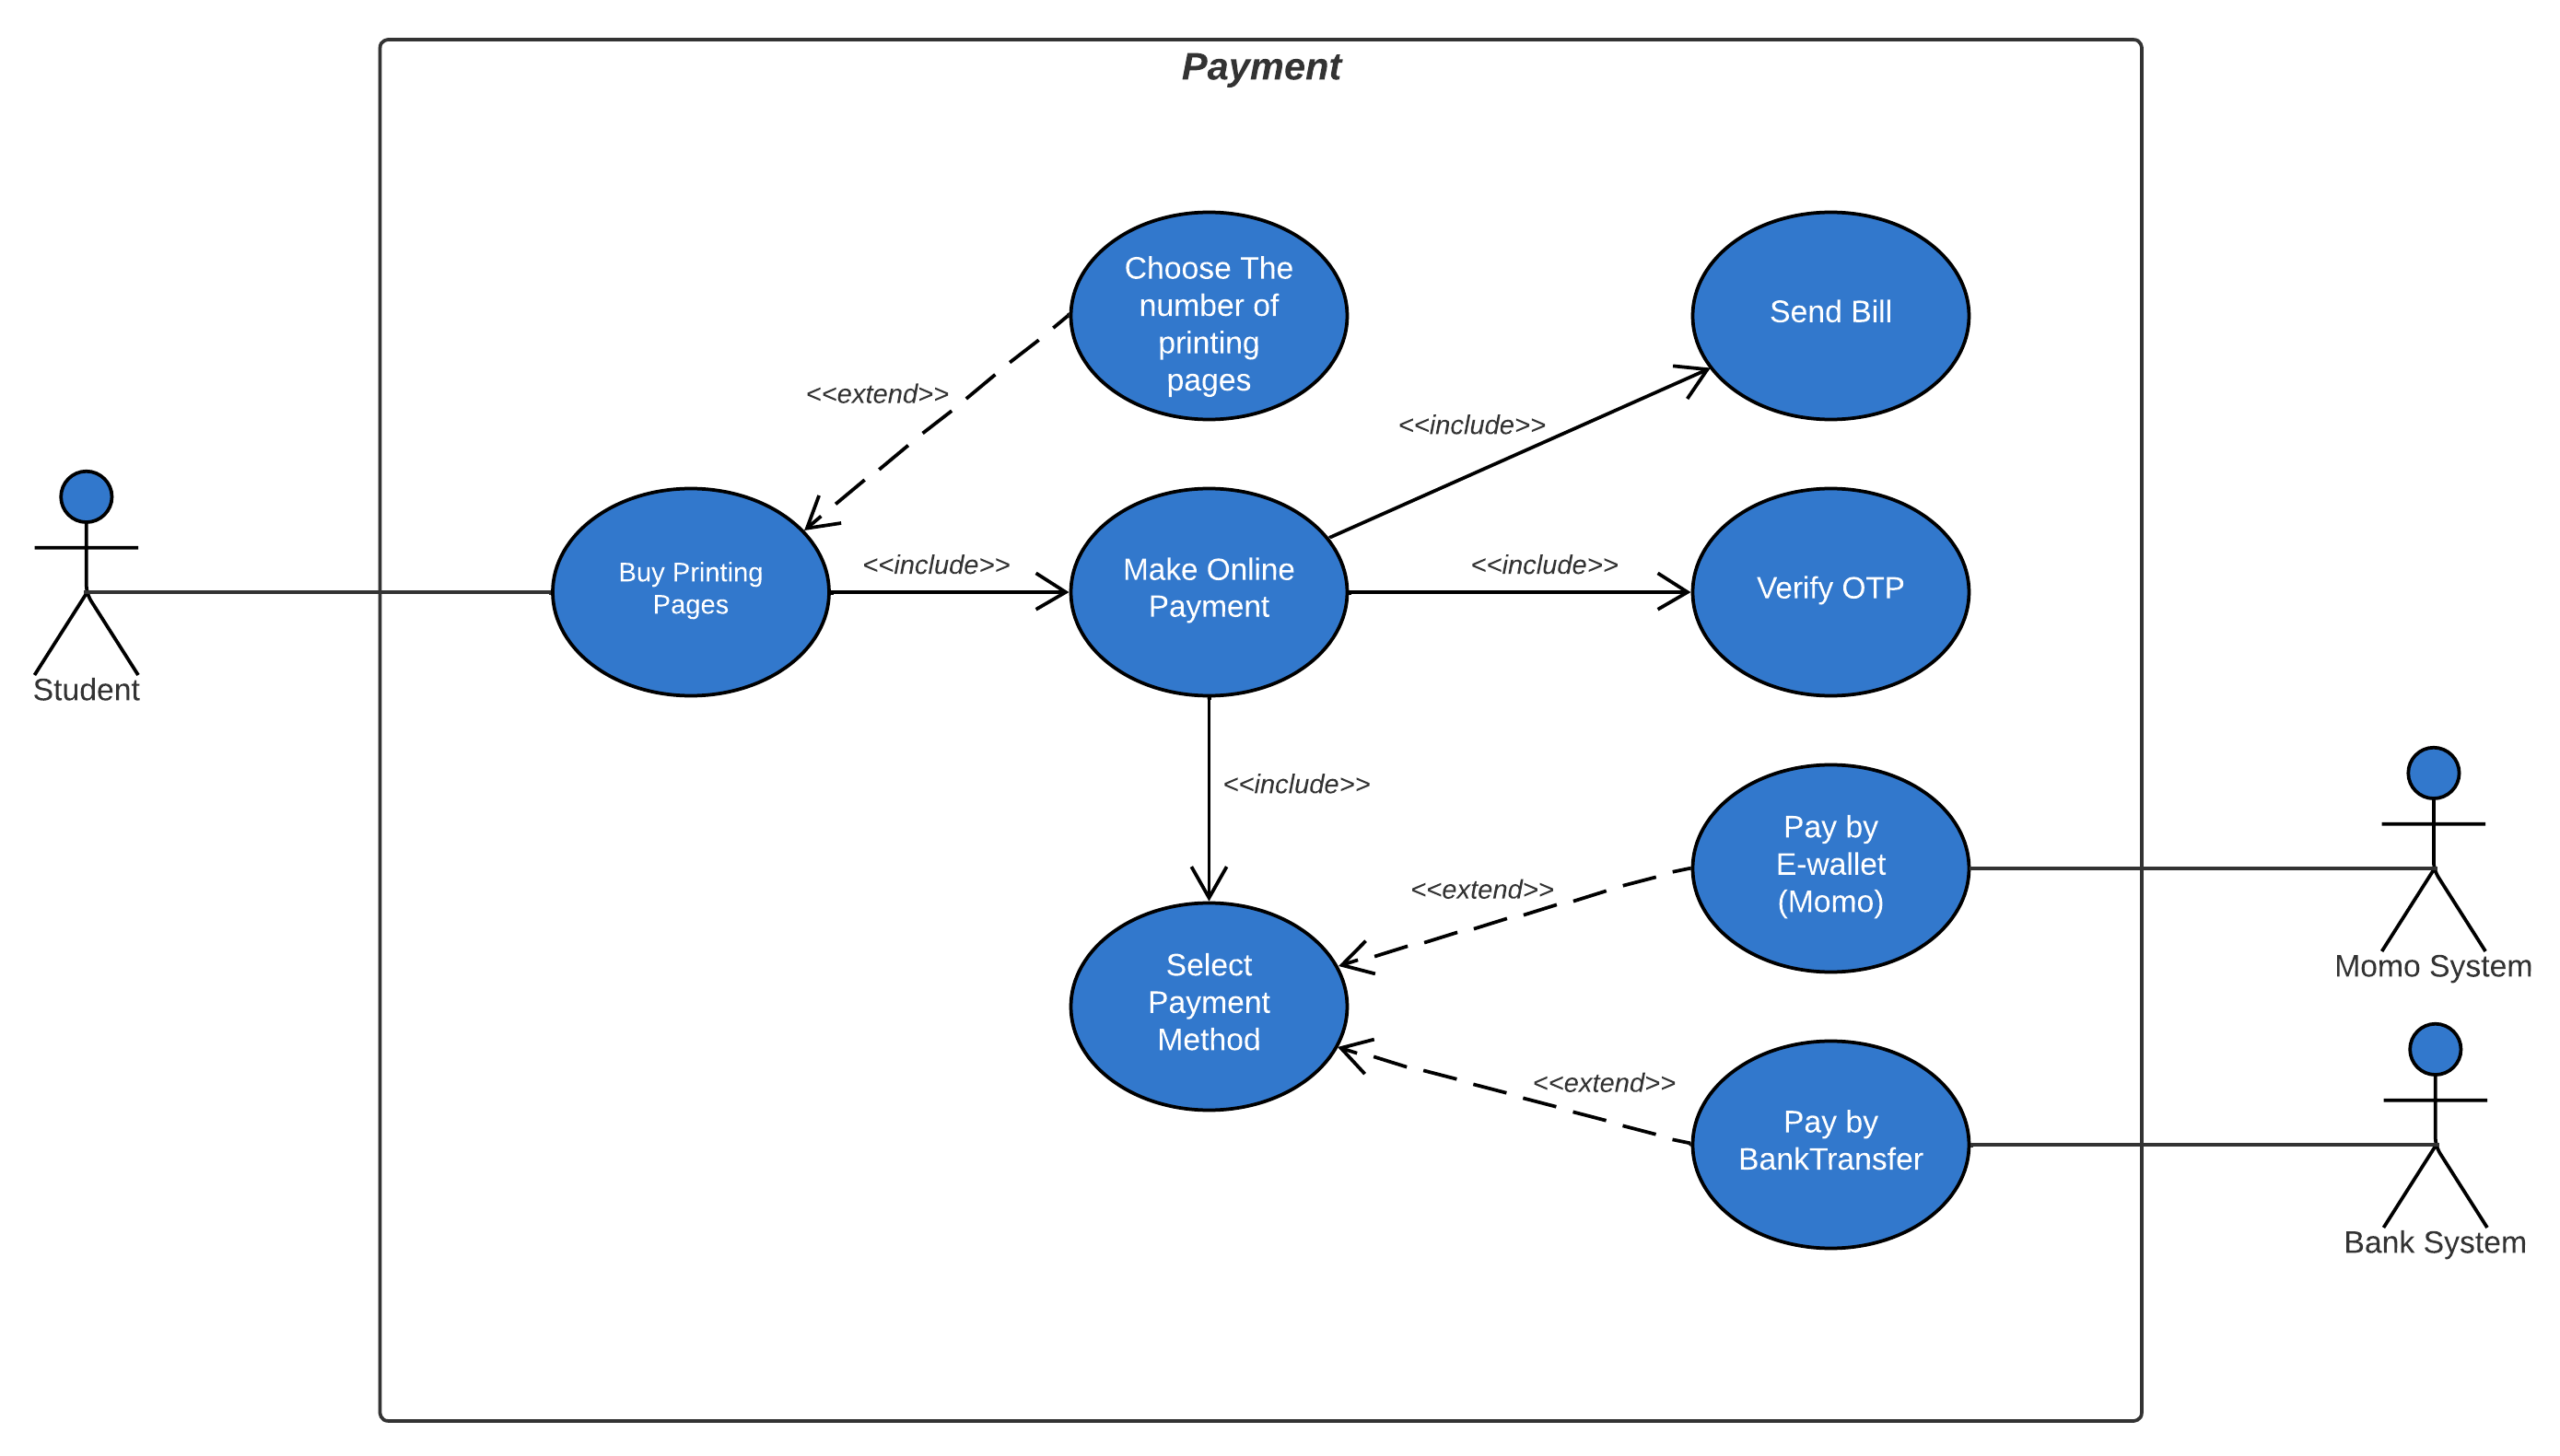
\includegraphics[scale=.62]{images/Task1/payment.png}
    \end{center}
    \label{refhinh1}
    \end{figure}
    \end{center}

    \begin{longtable}{|l|p{10cm}|}
        \hline
        \endhead
        \hline
        \endfoot
        Use-case Name & \textbf{Payment}\\
        \hline
        Actors & Sinh viên, Dịch vụ thanh toán (Hệ thống ngân hàng/ Hệ thống ví điện tử Momo).\\
        \hline
        Description & Use case này mô tả quá trình thanh toán cho giấy in được chọn bởi người dùng. Quá trình này bao gồm lựa chọn số lượng giấy in, cung cấp thông tin thanh toán, xác thực và xử lý thanh toán, sau đó người dùng nhận được xác nhận hoặc biên lai thanh toán.\\
        \hline
        Trigger & Sinh viên nhấn vào nút "Mua giấy in"\\
        \hline
        Pre-conditions & Sinh viên đã đăng nhập vào hệ thống thành công.\\
        \hline
        Post-conditions & - Cập nhật số lượng giấy in của sinh viên.\\
        & - Tài khoản sinh viên bị trừ số tiền tương ứng với số đã thanh toán.\\
        & - Đơn hàng được ghi nhận và lưu trữ.\\
        \hline
        Basic Flow & 1. Sinh viên nhấn vào nút "Mua giấy in".\\
        & 2. Sinh viên chọn số lượng trang giấy cần mua.\\
        & 3. Hệ thống tính toán tổng số tiền cần thanh toán dựa trên số lượng trang và giá in hiện tại.\\
        & 4. Sinh viên chọn phương thức thanh toán từ danh sách các phương thức có sẵn (ví điện tử, chuyển khoản ngân hàng).\\
        & 5. Sinh viên cung cấp chi tiết thanh toán cho phương thức đã chọn.\\
        & 6. Hệ thống gửi yêu cầu thanh toán đến Dịch vụ thanh toán.\\
        & 7. Dịch vụ thanh toán xử lý thanh toán và trả kết quả về cho hệ thống.\\
        & 8. Hệ thống cập nhật số lượng giấy in còn lại của sinh viên và trừ số tiền tương ứng từ tài khoản của họ.\\
        & 9. Đơn hàng được ghi nhận và lưu trữ trong hệ thống.\\
        & 10. Hệ thống hiển thị xác nhận mua thành công và biên lai thanh toán cho sinh viên.\\
        \hline
        Alternative Flow & Alternative 1: Sau bước 6, nếu thanh toán bị sai thông tin:\\
        & \hspace{1em} 6a.1. Hệ thống báo lỗi về thanh toán \\
        & \hspace{1em} 6a.2. Sinh viên ấn vào nút "Thanh toán lại".\\
        &\hspace{1em} Use case quay trở lại bước 6.
        \\
        \hline
        Exception Flow & Exception 1: Nếu sau bước 6, số tiền trong tài khoản sinh viên không đủ:\\
        & \hspace{1em} 6b.1. Hiển thị thông báo thanh toán thất bại.\\
        &\hspace{1em} Use case dừng lại.\\
        &\\
        & Exception 2: Nếu sau bước 10, nếu sinh viên không nhận được xác nhận hoặc biên lai thanh toán: \\
        & \hspace{1em} 10.1. Hệ thống cung cấp cách truy cập lại thông tin thanh toán để sinh viên kiểm tra lại.\\
        &\hspace{1em} Use case dừng lại.\\
        &\\
        & Exception 3: Nếu sau bước 6a.2, nếu sinh viên ấn vào nút "Hủy" thì hủy dịch vụ mua và trở về trang chủ.\\
        &\hspace{1em} Use case dừng lại.\\
    \end{longtable}
    
    \newpage
    \item{\textbf{Manage Printers}}
    \begin{center}
    \begin{figure}[htp]
    \begin{center}
     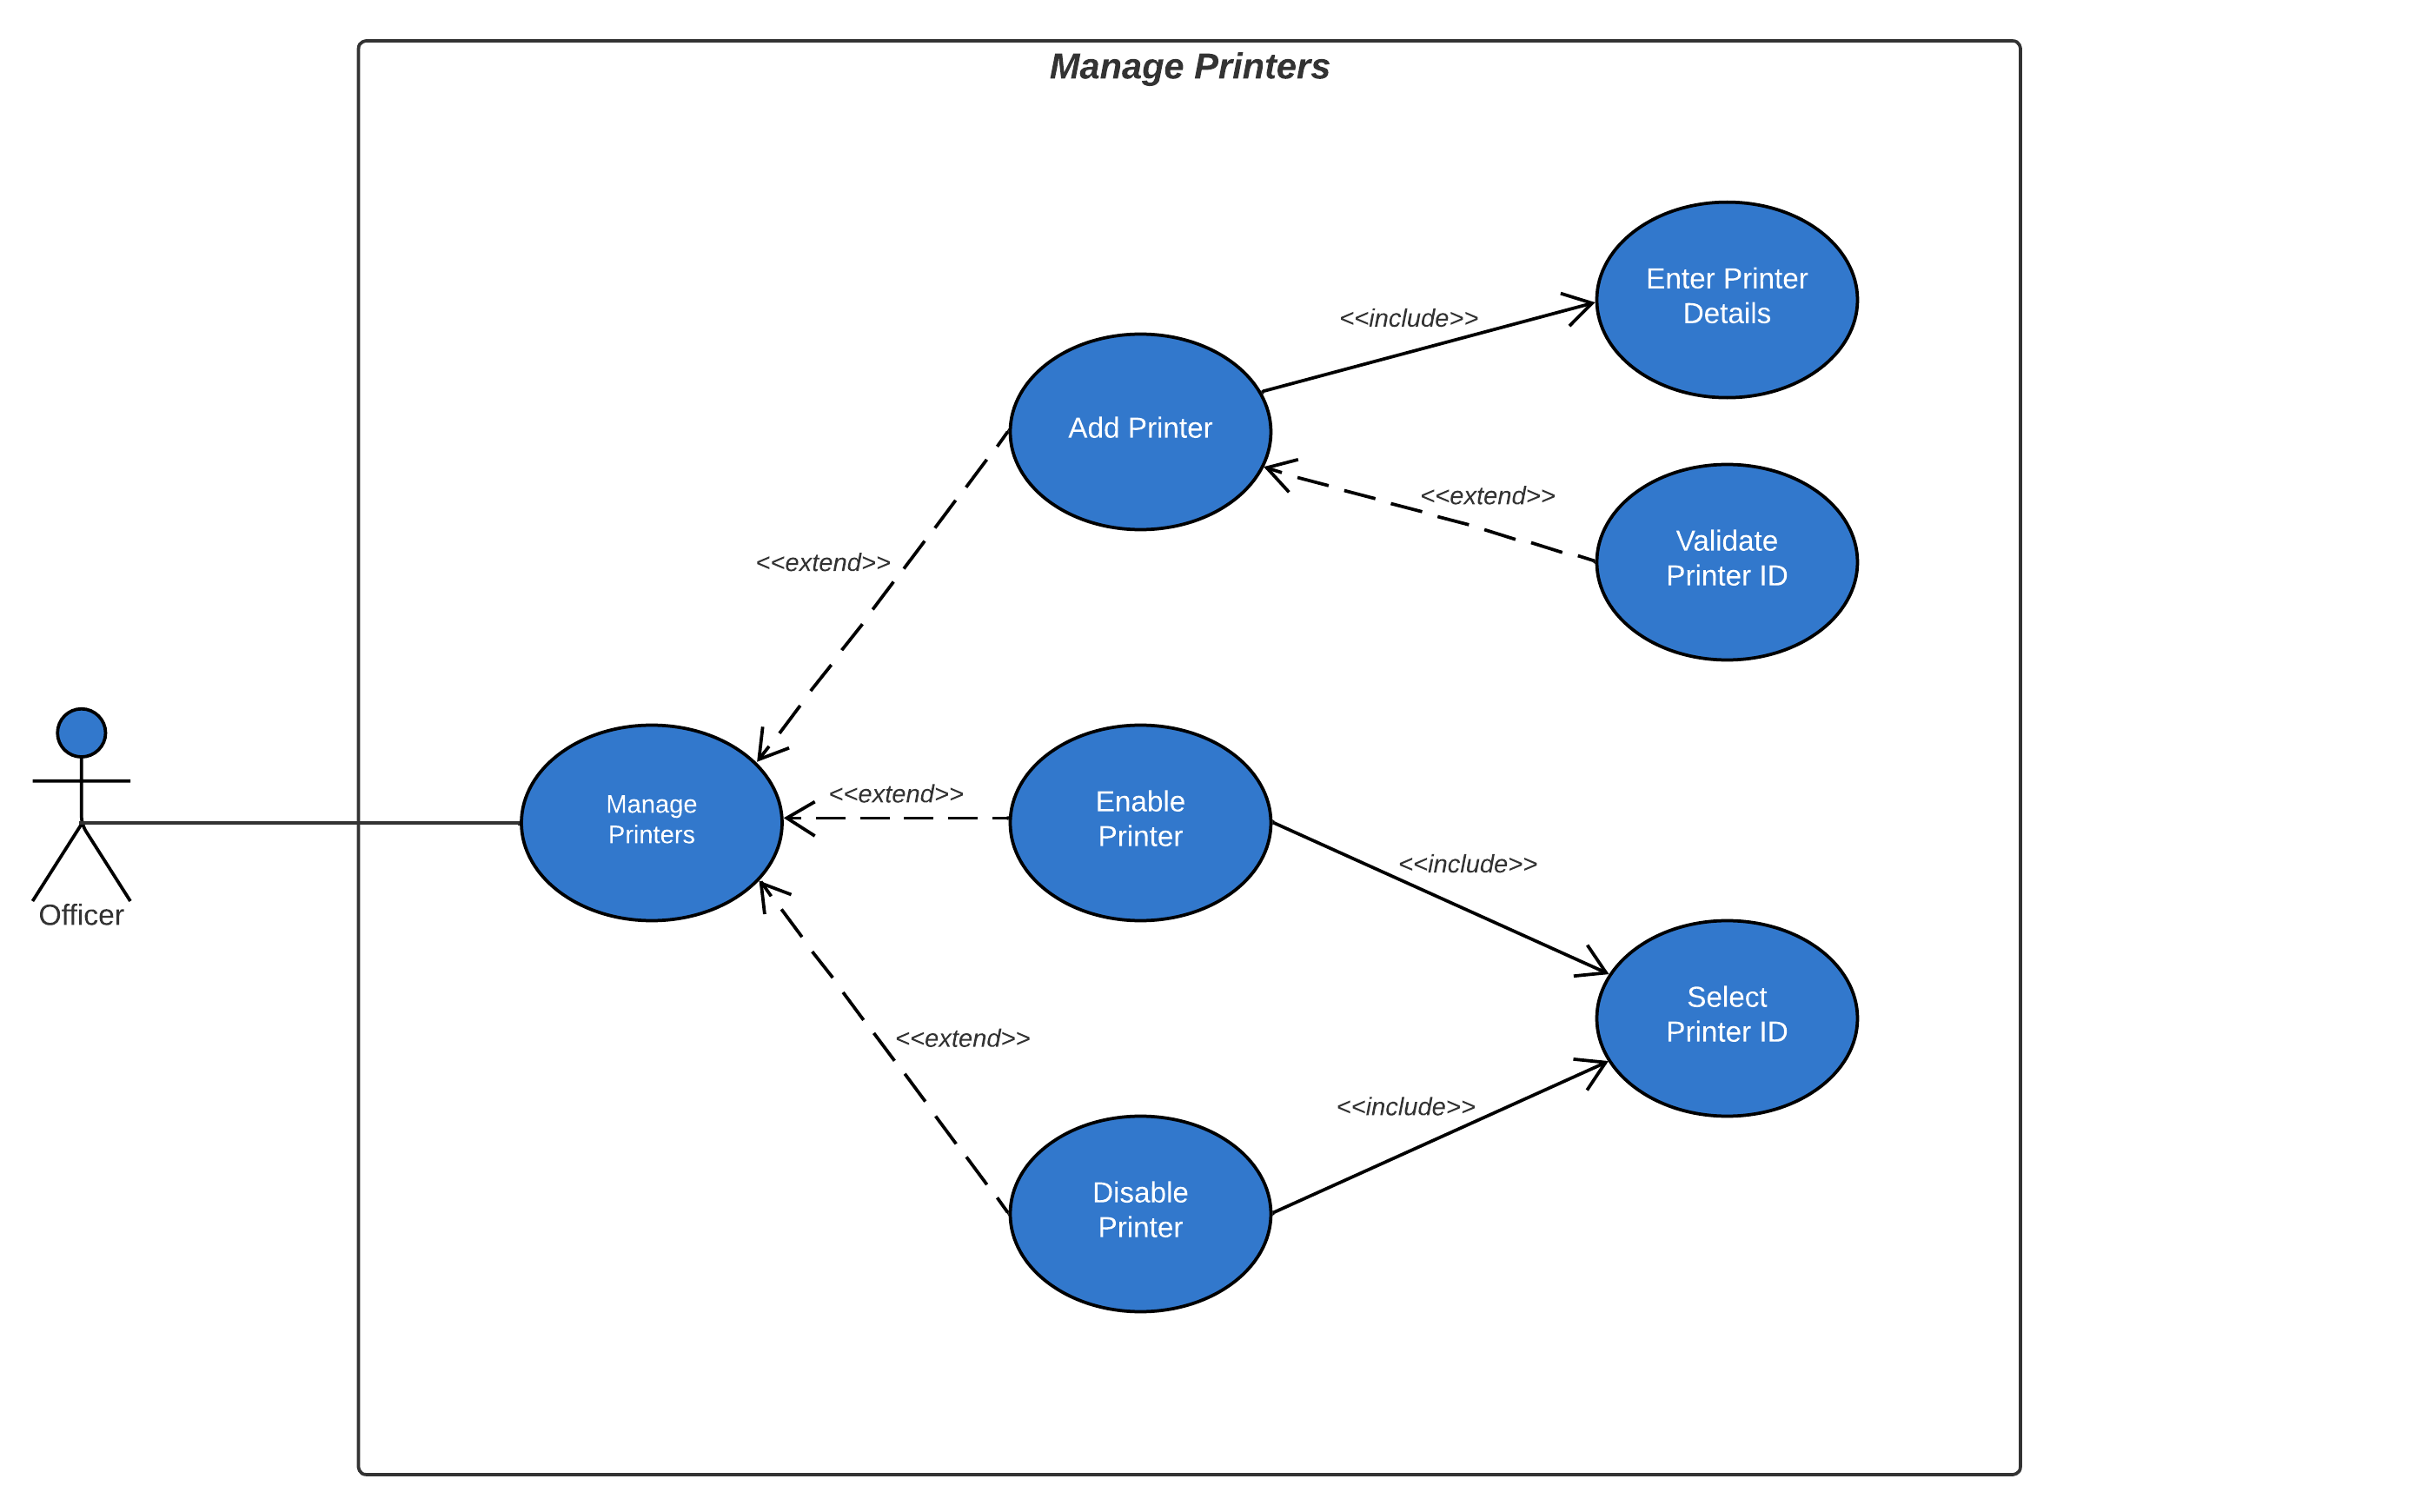
\includegraphics[scale=.62]{images/Task1/managePrinters.png}
    \end{center}
    \label{refhinh1}
    \end{figure}
    \end{center}

    \begin{longtable}{|l|p{10cm}|}
        \hline
        \endhead
        \hline
        \endfoot
        Use-case Name & \textbf{Manage Printers}\\
        \hline
        Actors & Student Printing Service Officer (SPSO) \\
        \hline
        Description & SPSO có thể quản lý các máy in qua những hành động như thêm máy in, bật máy in, tắt máy in và thay đổi cấu hình máy in.
        \\
        \hline
        Trigger 
            & - Lắp đặt thêm máy in: Khi trường đại học lắp đặt thêm máy in, SPSO có trách nhiệm thêm máy in đó vào hệ thống SPSS. \\
            & - Bảo trì máy in: Khi máy in có sự cố, SPSO tắt máy in, tạm thời loại máy in ra khỏi hệ thống đang hoạt động để kiểm tra, sửa chữa. Khi đã hoàn tất, SPSO có thể bật máy in và thêm vào hệ thống máy in đang hoạt động.
        \\
        \hline
        Pre-conditions &  
            - Người dùng (SPSO) phải được xác thực thông qua hệ thống đăng nhập HCMUT\_SSO. \\ &
            - SPSO phải có quyền truy cập vào hệ thống quản lý máy in. \\ &
            - Mỗi máy in chỉ được phép có một ID duy nhất (không trùng lặp). \\ &
            - Máy in phải có ID đang hoạt động trong hệ thống để bật hoặc tắt. \\ &
            - Hệ thống máy in đang hoạt động.
        \\
        \hline
        Post-conditions & None.\\
        \hline
        Basic Flow & 
            1. SPSO đăng nhập vào hệ thống quản lý máy in qua HCMUT\_SSO. \\ &
            2. SPSO chọn một trong ba chức năng: Thêm máy in, bật máy in, tắt máy in.
        \\
        \hline
        Alternative Flow & Alternative 1: Sau bước 2, nếu SPSO chọn chức năng thêm máy in:\\
        & \hspace{1em} 2a.1. SPSO xác nhận máy in vật lý đã được lắp đặt và kết nối điện.\\
        & \hspace{1em} 2a.2. SPSO sẽ gán một ID cố định cho máy in\\
        & \hspace{1em} 2a.3. SPSO sẽ đưa các hiệu chỉnh mặc định của hệ thống vào trong máy in.\\
        & \hspace{1em} 2a.4. SPSO sẽ điền các thông tin của máy in vào hệ thống (tên máy in, địa điểm, ...).\\
        &\\
        &Alternative 2: Sau bước 2, nếu SPSO chọn chức năng tắt máy in:\\
        & \hspace{1em} 2b.1. SPSO xác nhận máy in thông qua ID của máy in đó.\\
        & \hspace{1em} 2b.2. SPSO loại máy in đó khỏi hệ thống SPSS.\\
        &\\
        &Alternative 3: Sau bước 2, nếu SPSO chọn chức năng tắt máy in:\\
        & \hspace{1em} 2c.1. SPSO xác nhận máy in thông qua ID của máy in đó.\\
        & \hspace{1em} 2c.2. SPSO thêm lại máy in đó vào hệ thống SPSS.\\
        \hline
        Exception Flow & Exception 1: SPSO có thể chọn lại ID nếu ID ban đầu không đúng với máy in cần thêm / bớt hoặc ID không tồn tại\\
        &\\
         & Exception 2: SPSO có thể gán lại ID cho máy in mới nếu ID được chọn đã tồn tại sẵn trong hệ thống.\\
    \end{longtable}
    
    \newpage
    \item{\textbf{Configure System}}
    \begin{center}
    \begin{figure}[htp]
    \begin{center}
     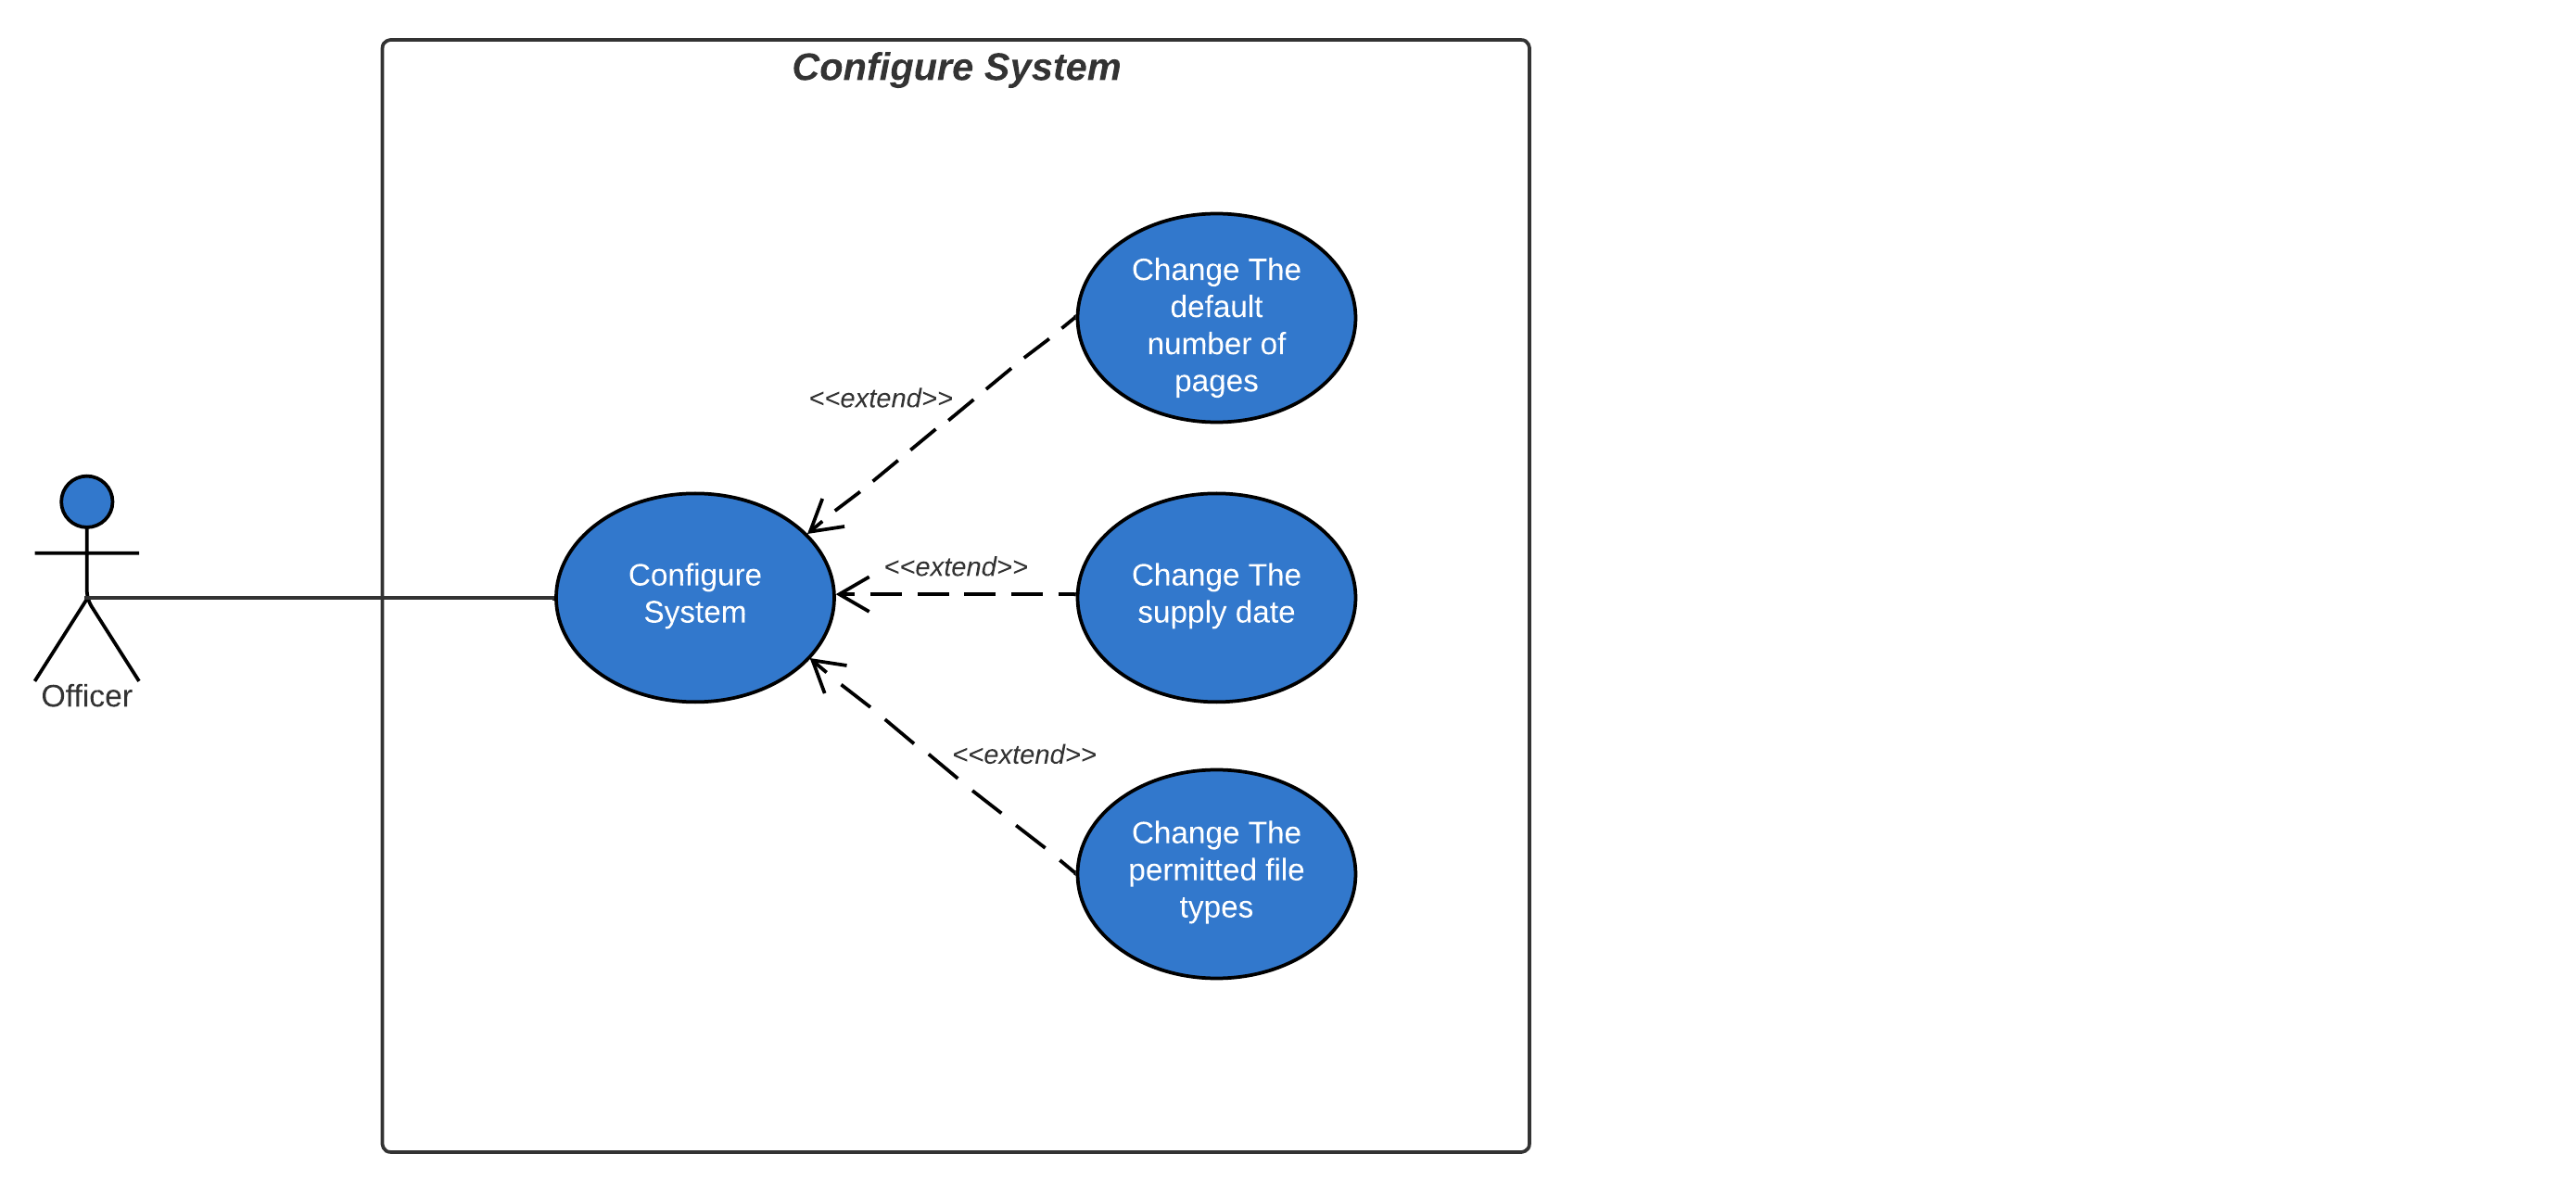
\includegraphics[scale=.62]{images/Task1/configureSystem.png}
    \end{center}
    \label{refhinh1}
    \end{figure}
    \end{center}

    \begin{longtable}{|l|p{10cm}|}
        \hline
        \endhead
        \hline
        \endfoot
        Use-case Name & \textbf{Configure System}\\
        \hline
        Actors & Student Printing Service Officer (SPSO)\\
        \hline
        Description & SPSO có quyền thay đổi các tùy chỉnh của hệ thống bao gồm số lượng tờ giấy mặc định, thời điểm mà hệ thống cung cấp cho tất cả sinh viên một số lượng giấy in mặc định, các định dạng tập tin được chấp nhận bởi hệ thống.\\
        \hline
        Trigger & Khi SPSO chọn chức năng Configure system trong trang chính của phần mềm quản lý hệ thống máy in.\\
        \hline
        Pre-conditions & SPSO phải đăng nhập thành công vào hệ thống\\
        \hline
        Post-conditions & - Giao diện để thay đổi các tùy chỉnh của hệ thống sẽ hiện lên.\\
        & - SPSO cập nhật thành công số lượng giấy in mặc định, thời điểm mà hệ thống cung cấp cho tất cả sinh viên một số lượng giấy in mặc định, các định dạng tập tin được chấp nhận bởi hệ thống.\\
        \hline
        Basic Flow & 1. SPSO đăng nhập vào hệ thống quản lý máy in HCMUT\_SSO\\
        & 2. SPSO chọn chức năng Configure system trong trang chính của phần mềm quản lý hệ thống máy in.\\
        & 3. SPSO chọn một trong ba chức năng: tùy chỉnh số lượng giấy in mặc định, tùy chỉnh thời điểm hệ thống cung cấp cho tất cả sinh viên một số lượng giấy in mặc định hoặc tùy chỉnh các định dạng tập tin được chấp nhận bởi hệ thống.\\
        & 4. Trong trang chức năng, SPSO nhấn nút lưu để cập nhật thông tin được thay đổi, một bảng thông báo "Cập nhật thành công" sẽ hiện lên, SPSO nhấn nút OK để tắt.\\
        \hline
        Alternative Flow & Alternative 1: Sau bước 3, Nếu SPSO chọn chức năng tùy chỉnh số lượng giấy in mặc định.\\
        & \hspace{1em} 3a.1. SPSO có thể nhập số lượng giấy in mặc định mới. \\
        & \hspace{1em} 3a.2. SPSO nhấn nút lưu để cập nhật thay đổi.\\
        
        &Alternative 2: Sau bước 3, Nếu SPSO chọn chức năng tùy chỉnh thời điểm hệ thống cung cấp cho tất cả sinh viên một số lượng giấy in mặc định:\\
        & \hspace{1em} 3b.1. SPSO có thể thay đổi các thông số của thời điểm nêu trên bao gồm giờ, phút, giây, ngày, tháng và năm thông qua các drop down list.\\
        & \hspace{1em} 3b.2. SPSO bấm nút lưu để cập nhật thay đổi.\\
        &\\
        &Alternative 3: Sau bước 3, Nếu SPSO chọn chức năng tùy chỉnh các định dạng tập tin được chấp nhận bởi hệ thống:\\
        & \hspace{1em} 3c.1. SPSO thêm hoặc xóa bớt một định dạng tập tin trong danh sách các tập tin được hệ thống chấp nhận.\\
        & \hspace{1em} 3c.2. SPSO bấm nút lưu để cập nhật thay đổi.\\
        \hline
        Exception Flow & Exception 1: Sau bước 2, SPSO có thể nhấn nút quay lại để trở về trang chính của phần mềm quản lý hệ thống máy in.\\
        &\\
        & Exception 2: Sau bước 3, SPSO có thể nhấn nút hủy để quay lại màn hình chọn chức năng cần tùy chỉnh.\\
        &\\
        & Exception 3: Ở luồng sự kiện phụ 3a.1, nếu SPSO nhập số lượng giấy in không hợp lệ và nhấn lưu, một bảng thông báo "số lượng giấy in không hợp lệ" sẽ hiện lên, SPSO nhấn nút OK để quay lại luồng sự kiện phụ 3a.1.\\
        &\\
        & Exception 4: ở luồng sự kiện phụ 3c.1, nếu SPSO thêm một định dạng tập tin không hợp lệ và nhấn lưu, một bảng thông báo "định dạng không hợp lệ" sẽ hiện lên, SPSO nhấn nút OK để quay lại luồng sự kiện phụ 3c.1\\
    \end{longtable}

    
    \newpage
    \item{\textbf{Log In}}
    \begin{center}
    \begin{figure}[!htp]
    \begin{center}
     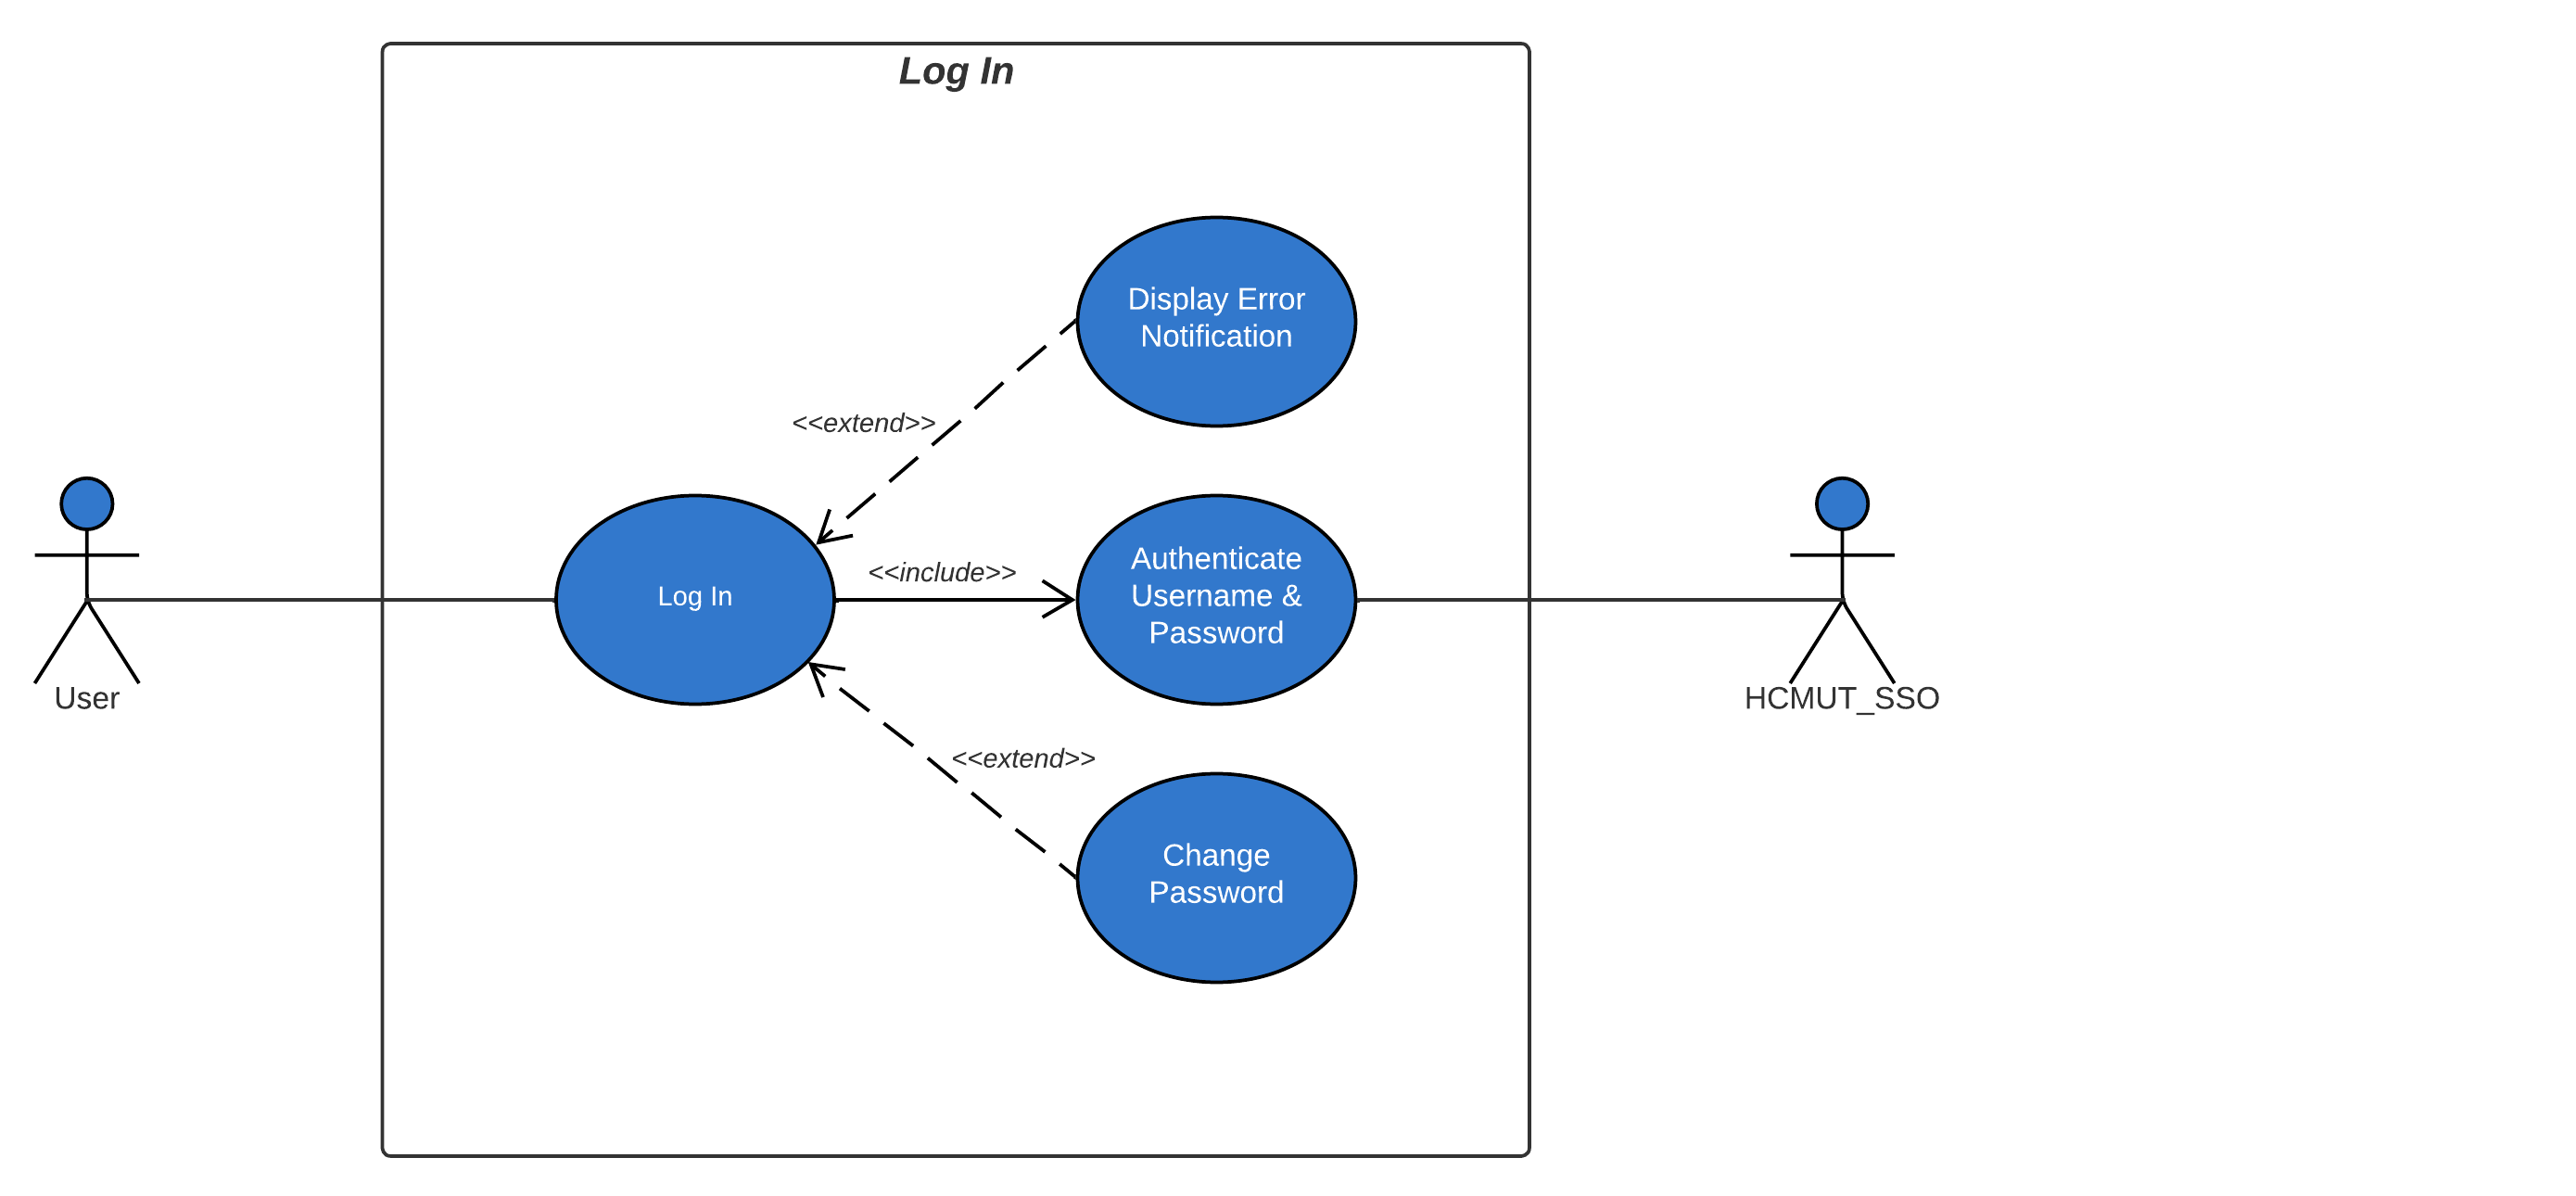
\includegraphics[scale=.62]{images/Task1/login.png}
    \end{center}
    \label{refhinh1}
    \end{figure}
    \end{center}

    \begin{longtable}{|l|p{10cm}|}
        \hline
        \endhead
        \hline
        \endfoot
        Use-case Name & \textbf{Log In}\\
        \hline
        Actors & Sinh viên, Student Printing Service Officer. \\
        \hline
        Description & Người dùng thực hiện việc đăng nhập vào hệ thống.\\
        \hline
        Trigger & Người dùng truy cập trang đăng nhập và bắt đầu nhập thông tin đăng nhập.\\
        \hline
        Pre-conditions & - Tài khoản của người dùng đã được tạo.\\
                       & - Tài khoản của người dùng đã được phân quyền.\\
                       & - Thiết bị của người dùng đã được kết nối internet khi thực hiện đăng nhập.\\
        \hline
        Post-conditions & Người dùng đăng nhập thành công và có thể sử dụng những chức năng của hệ thống\\
        \hline
        Basic Flow & 1. Người dùng truy cập trang đăng nhập.\\
        & 2. Người dùng nhập tài khoản và mật khẩu.\\
        & 3. Hệ thống xác thực thông tin đăng nhập thành công và cho phép người dùng truy cập ứng dụng.\\
        & 4. Hệ thống ghi nhận hoạt động đăng nhập thành công \\
        \hline
        Alternative Flow & None.\\
        \hline
        Exception Flow & Exception 1: Ở bước 3, nếu tài khoản hoặc mật khẩu sai:\\
        & \hspace{1em} 3.1. Hệ thống hiển thị thông báo sai tài khoản hoặc mật khẩu.\\
        & \hspace{1em} 3.2. Hệ thống quay về trang đăng nhập. \\
        &\hspace{1em} Use case dừng lại.\\
        
        & Exception 2: Sau bước 1, nếu người dùng chọn đổi mật khẩu:\\
        & \hspace{1em} 1.1. Hiển thị trang đổi mật khẩu bao gồm 4 trường nhập tài khoản, nhập mật khẩu cũ, nhập mật khẩu mới và xác nhận mật khẩu mới. \\
        & \hspace{1em} 1.2. Nếu thông tin đúng thì mật khẩu được thay đổi.\\
        &\hspace{1em} Use case dừng lại.\\
    \end{longtable}
    \end{enumerate}